\documentclass[12pt]{article}
% Chinese Support
\usepackage{xeCJK}
\setCJKmainfont{STSong}
% \setmainfont{Times New Roman}

\usepackage{float}

% for symbol
\usepackage{gensymb}
% matrix
\usepackage{amsmath}

% For images
\usepackage{graphicx}
\graphicspath{ {./screenshoot/} }

\newcommand{\numpy}{{\tt numpy}}    % tt font for numpy

\topmargin -1.in
\textheight 9in
\oddsidemargin -.25in
\evensidemargin -.25in
\textwidth 7in


\usepackage{listings}
\usepackage{color}
\usepackage{xcolor}

\definecolor{dkgreen}{rgb}{0,0.6,0}
\definecolor{gray}{rgb}{0.5,0.5,0.5}
\definecolor{mauve}{rgb}{0.58,0,0.82}
\definecolor{textblue}{rgb}{.2,.2,.7}
\definecolor{textred}{rgb}{0.77,0,0}
\definecolor{textgreen}{rgb}{0,0.43,0}

% \setmonofont{FiraCode-Regular}
\lstset{frame=tb,
  language=C++,
  aboveskip=3mm,
  belowskip=3mm,
  showstringspaces=false,
  columns=flexible,
  basicstyle={\ttfamily},
  numbers=none,
  numberstyle=\tiny\color{gray},
  keywordstyle=\color{blue}\itshape,
  stringstyle=\color{mauve},
  breaklines=true,
  breakatwhitespace=true,
  commentstyle=\color{textred}\itshape,
  tabsize=3
}



% Content start below
\begin{document}

\author{陈铭涛\\16340024}
\title{计算机图形学 Homework 8 - Bézier Curve}
% \date{\vspace{-5ex}}
\maketitle

\medskip

% ========== Begin answering questions here

\section{Basic}

\begin{enumerate}
    \item 用户能通过左键点击添加Bezier曲线的控制点,右键点击则对当前添加的最后一个控制点进行消除
    \item 工具根据鼠标绘制的控制点实时更新Bezier曲线。
    

    Bézier 曲线的参数方程如下:
    \begin{equation}
        \begin{aligned}
        Q(t) = \sum_{i=0}^{n}P_iB_{i, n}(t), t\in[0, 1]
        \end{aligned}
    \end{equation}
    其中$B_{i, n}(t)$为伯恩斯坦基函数,多项式表示为:
    \begin{equation}
        \begin{aligned}
        B_{i, n}(t) = \frac{n!}{i!(n-i)!}t^i(1-t)^{n-i}, i=0,1...n
        \end{aligned}
    \end{equation}
    代码中的实现如下:
    \begin{lstlisting}
        float t_step = 1.0 / steps;
        int n = points.size() - 1;
        for (int k = 0; k <= steps; k++) {
            glm::vec3 current_point = {0, 0, 0};
            for (int i = 0; i <= n; i++) {
                current_point += points[i] * float(bernstein(i, n, t_step * k));
            }
            result.push_back(current_point);
        }
    \end{lstlisting}

    GLFW 下获取鼠标点击的方法为通过 \lstinline{glfwSetMouseButtonCallback} 设置鼠标操作时的回调函数,对左键和右键的 \lstinline{GLFW_PRESS} 操作进行处理,当按下左键时添加控制点,按下右键时去除一个控制点。

    获得的具有4个控制点的3阶贝塞尔曲线如下:

    \begin{figure}[H]
        \centering
        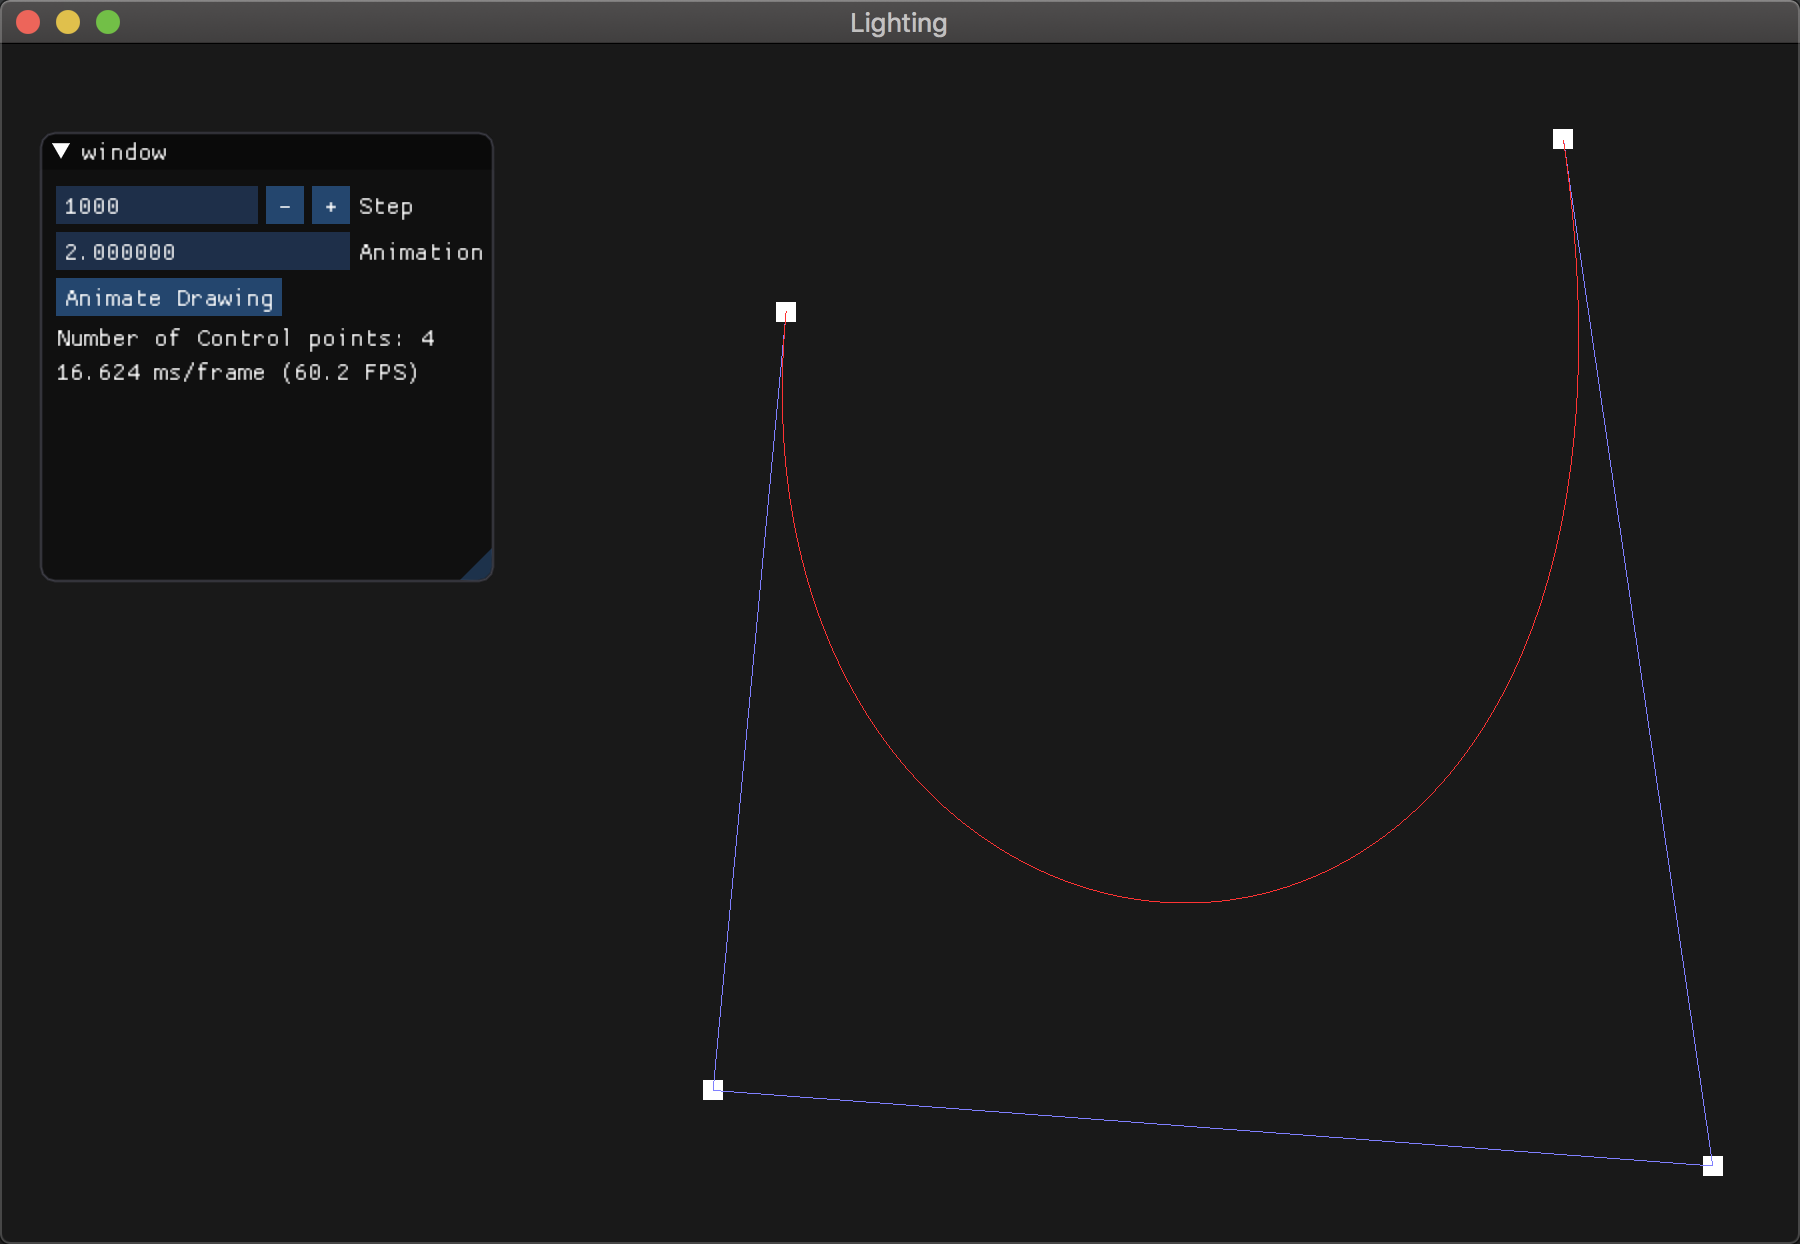
\includegraphics[scale=0.5]{cubic.png}
        \caption{三次贝塞尔曲线}
        \label{}
    \end{figure}

    通过鼠标控制点实时更新贝塞尔曲线的效果请见 demo。
\end{enumerate}


\section{Bonus}
\begin{enumerate}
    \item 可以动态地呈现Bezier曲线的生成过程。
    
    $n$阶贝塞尔曲线为两个$n-1$阶贝塞尔曲线的插值,因此动态显示贝塞尔曲线的生成过程的方法为从$n=1$开始插值获得$n$阶的曲线。

    例子如下:

    对于3个控制点的贝塞尔曲线:
    \begin{enumerate}
        \item 1 次时获得三个控制点间的两条曲线:
        $$B_{1,1}(t)=P_0(1-t)+P_1t$$
        $$B_{1,2}(t)=P_1(1-t)+P_2t$$

        \item 对两条 1 次曲线进行插值,获得2次曲线:
        $$B_{2,1}(t)=B_{1,1}(t)(1-t)+B_{1,2}(t)t$$
        展开得
        $$B_{2,1}(t)=P_0(1-t)^2+2P_1t(1-t)+P_2t^2$$
        即 2 次贝塞尔曲线,由此将过程中每步进行1次插值的结果绘出即可显示出 Bezier 曲线的生成过程。
        
    \end{enumerate}

    对6个控制点的贝塞尔曲线生成过程进行显示的效果如下:
    \begin{figure}[H]
        \centering
        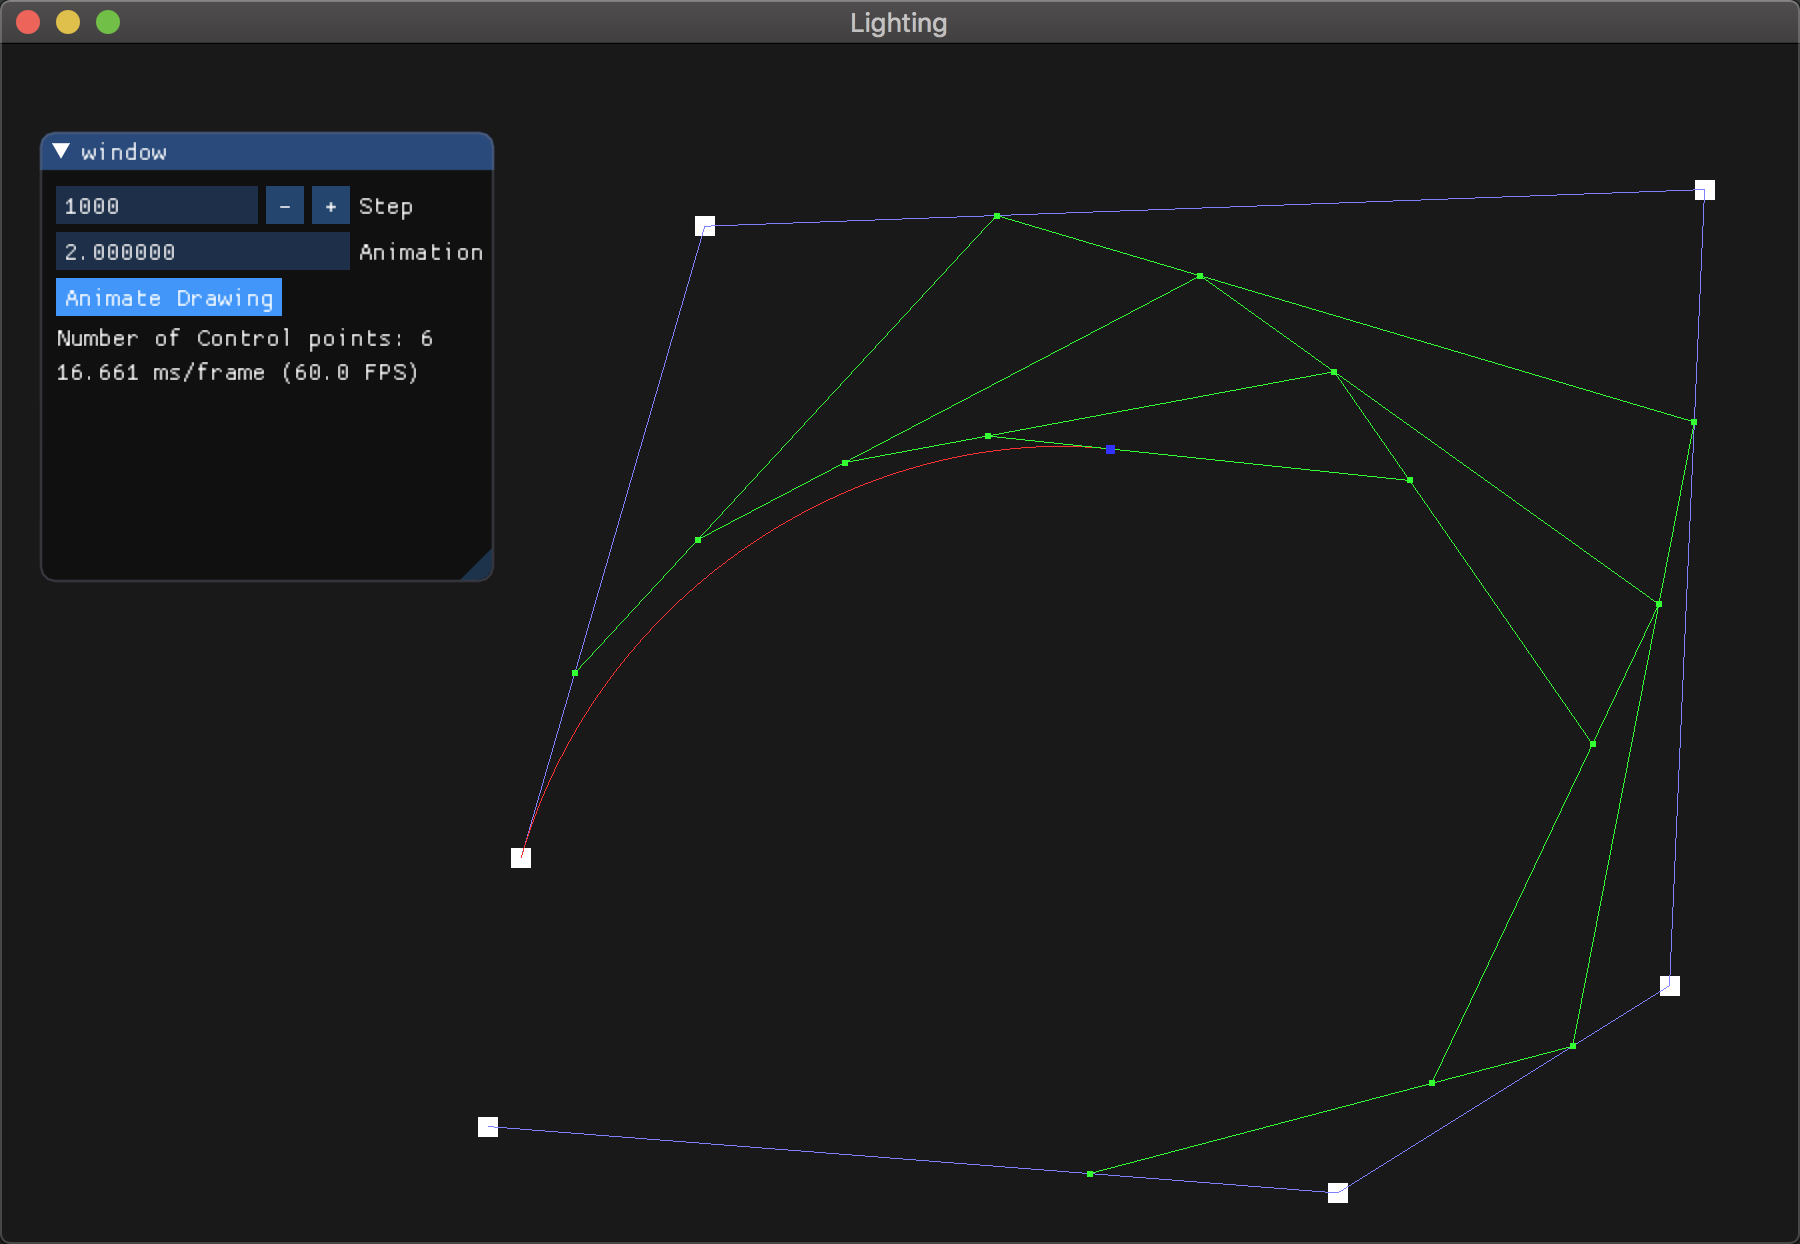
\includegraphics[scale=0.5]{dyn.png}
        \caption{贝塞尔曲线生成过程}
        \label{}
    \end{figure}

    具体的动态效果请见 demo。
\end{enumerate}
        





\end{document}
\grid
\grid
